% Exploratory case studies are used as initial investigations of some phenomena to derive new hypotheses and build theories~\cite{easterbrook2008selecting}
% "A multiple case study offers greater validity"~\cite{easterbrook2008selecting}

% Summary of cases: Business sector, ML domain, Target Platform

\DIFdelbegin %DIFDELCMD < \begin{table}[ht]
%DIFDELCMD <   %%%
\DIFdelendFL \DIFaddbeginFL \begin{table}
  \DIFaddendFL \caption{Summary of ML cases}
    \DIFdelbeginFL %DIFDELCMD < \resizebox{\columnwidth}{!}{
%DIFDELCMD <     \begin{tabular}{lp{2,2cm}p{3cm}p{1.2cm}l} 
%DIFDELCMD <         \textbf{Case} & \textbf{Sector} & \textbf{ML Task} & \textbf{Platform}\\ 
%DIFDELCMD <         \hline
%DIFDELCMD <         1 &  Advertising       & Ad Targeting    & Cloud  \\ % smartly helsinki
%DIFDELCMD <         2 &  Gaming     & Object detection and OCR   & Cloud  \\ % Noice
%DIFDELCMD <         3 &  Healthcare    & Transcription & Cloud  \\ % Inscripta
%DIFDELCMD <         4 &  Financial Services    & Risk Modelling & Cloud  \\ % Aktia
%DIFDELCMD <         5 &  Financial Services    & OCR   & Cloud \\ %Baseware
%DIFDELCMD <         6 &  Software Platform & Multiple ML Tasks & Cloud/IoT \\ % SoftwareAG
%DIFDELCMD <         7 &  Advertising & Ad Optimization  & Cloud \\ % Smartly california
%DIFDELCMD <         8 &  Manufacturing & Anomaly Detection & Edge \\ % Siemens
%DIFDELCMD <         \hline    
%DIFDELCMD <         \end{tabular}
%DIFDELCMD <     }
%DIFDELCMD <   %%%
\DIFdelendFL \DIFaddbeginFL \begin{tabular}{lp{3cm}p{3.5cm}p{2.0cm}p{3.2cm}l} 
        \textbf{\DIFaddFL{Case}} & \textbf{\DIFaddFL{Sector}} & \textbf{\DIFaddFL{ML Task}} & \textbf{\DIFaddFL{Platform}} & \textbf{\DIFaddFL{Interviewee Role}}\\ 
        \hline
        \DIFaddFL{1 }&  \DIFaddFL{Advertising       }& \DIFaddFL{Ad Targeting    }& \DIFaddFL{Cloud }& \DIFaddFL{ML Enginneers (2) }\\ %DIF >  smartly helsinki
        \DIFaddFL{2 }&  \DIFaddFL{Gaming     }& \DIFaddFL{Object detection and OCR   }& \DIFaddFL{Cloud  }& \DIFaddFL{ML Engineers (2) }\\ %DIF >  Noice
        \DIFaddFL{3 }&  \DIFaddFL{Healthcare    }& \DIFaddFL{Transcription }& \DIFaddFL{Cloud  }& \DIFaddFL{CTO}\\ %DIF >  Inscripta
        \DIFaddFL{4 }&  \DIFaddFL{Financial Services    }& \DIFaddFL{Risk Modelling }& \DIFaddFL{Cloud  }& \DIFaddFL{ML Engineer}\\ %DIF >  Aktia
        \DIFaddFL{5 }&  \DIFaddFL{Financial Services    }& \DIFaddFL{OCR   }& \DIFaddFL{Cloud }& \DIFaddFL{Senior Software Engineer}\\ %DIF > Baseware
        \DIFaddFL{6 }&  \DIFaddFL{Software Platform }& \DIFaddFL{Multiple ML Tasks }& \DIFaddFL{Cloud/IoT }& \DIFaddFL{Product Manager}\\ %DIF >  SoftwareAG
        \DIFaddFL{7 }&  \DIFaddFL{Advertising }& \DIFaddFL{Ad Optimization  }& \DIFaddFL{Cloud }& \DIFaddFL{ML Engineer}\\ %DIF >  Smartly california
        \DIFaddFL{8 }&  \DIFaddFL{Manufacturing }& \DIFaddFL{Anomaly Detection }& \DIFaddFL{Edge }& \DIFaddFL{ML Engineer}\\ %DIF >  Siemens
        \hline    
        \end{tabular}
  \DIFaddendFL \label{tab: ml_case_summary}
\end{table}
This study applies an exploratory multiple-case study research design approach \cite{runeson2009guidelines}. The multi-case study research methodology is used because of its suitability in exploring complex phenomena in their real context~\cite{easterbrook2008selecting, runeson2009guidelines}. Ethnographic methods like interviews are a common way to collect data for case studies, especially for studies in software engineering processes~\cite{giray2021software}. We conducted semi-structured interviews with practitioners across eight companies, similar to previous studies~\cite{shankar2022operationalizing, baier2019challenges, lwakatare2019taxonomy}.

\subsection{Research objectives}
As discussed in section~\ref{sec: background and related work}, empirical studies in AI engineering \cite{bosch2021engineering} tend to explore the entire ML workflow and further focus on identifying challenges encountered in various workflow stages. This study specifically focuses on the deployment and inference aspects of the ML/DL model in real-world production settings. That is, considering the process that begins when an ML/DL model is eventually ready for integration into the rest of the software ecosystem. Our goal is to capture patterns of practices applied in converting inference code into an inference service, which is the deployment procedure shown in Figure~\ref{fig:deployment_highlevel_framework}. We interviewed practitioners with hands-on experience deploying ML systems to achieve our objective. A summary of the ML systems, their respective deployment platforms and the case company's business sector is presented in Table~\ref{tab: ml_case_summary}. Our study seeks to answer the following questions:

% Image: an overview of the deployment process
\begin{figure}[h]
\centering
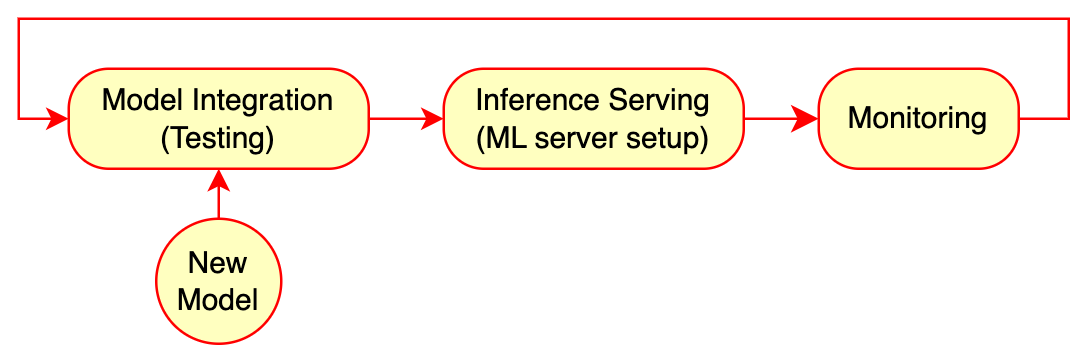
\includegraphics[width=0.5\textwidth]{deployment_highlevel_framework}
\caption{A high-level view of deployment activities}
\label{fig:deployment_highlevel_framework}
\end{figure}

\subsection{Research questions (RQ)}
\begin{itemize}
    \item RQ1) How are deployment workflows of ML/DL models implemented in production settings?
    \item RQ2) What patterns emerge in deployment workflows of ML/DL models?
    \item RQ3) How are inference architectures implemented?
\end{itemize}

\subsection{Case and Participant Selection}
% Unit of analysis?
A case in our multi-case study design approach represents an organization's deployed ML/DL system. By focusing on deployed production systems, we aimed to ensure the interviewee references a tried and tested workflow irrespective of its efficiency. Our goal was to be able to discuss the adopted approaches and, potentially, the rationale of various design decisions.
%The ML code has been deployed into production for an operational software application and service. 

After contacting several companies, we selected companies whose ML-enabled systems had been deployed to production. Three of the companies that responded had participated in our previous study~\cite{muiruri2022practices}, while five cases were new to us. Interviewees in this study were required to be actively involved in deploying the ML system. This was necessary to facilitate a richer discussion on the technology stack choice and potential improvement areas, among other architectural decisions.


\subsection{Data Collection}
Eight semi-structured interviews were conducted, and two researchers were present during the interview sessions. One practitioner from an organization was interviewed, except in one case where two practitioners were involved. The interview sessions were guided by the list of questions in Table~\ref{tab: interview_questions}. These questions were sent to the case companies before the interview. This ensured that the company identified a person with the relevant system knowledge to participate in the discussion. Five company interviews were conducted virtually through video conferencing, and one interview was conducted in a physical meeting, while two companies that were involved in our previous study participated through email correspondence since we were familiar with their solution. All data was gathered between September 2022 and November 2022. All interview discussions were recorded and transcribed for analysis.

Discussions with the interviewees did not strictly follow the order in the list of questions; instead, we probed the interviewee based on the breadth and depth of answers to a given query. Virtual interviews were recorded using zoom\footnote{https://zoom.us/} and transcribed using Otter.ai\footnote{https://otter.ai/}. We manually corrected any transcription errors that appeared before starting the analysis process.

 
\subsection{Data Analysis}
The transcribed text was the primary input for the analysis process. Using the deployment process text descriptions for each case, the two researchers extracted the activities in the deployment process and, at the same time, visualized the inference architecture of the entire ML system. A summary of the deployment process and the inference system architecture were sent via email to each case for validation as well as to get further clarifications. At this phase, researchers initially identified standard practices cross-cutting the cases. 

A systematic cross-case analysis~\cite{seaman1999qualitative} was conducted wherein using our interview questions (rows) and companies (columns), we formed a matrix~\cite{webster2002analyzing} and each response to a question by a given company was extracted, analyzed, and entered into a relevant cell in the matrix. Effectively, the matrix contained eight rows and six columns where a single cell represented a company and its approach to a given topical issue probed with a question. During this analysis process, any conceptual gaps identified in the responses were clarified with the interviewee through email correspondence. We synthesized an overall view for each row and summarised it as a topical deployment pattern.

% Table interview questions

\begin{table}
    %\fontsize{9pt}{8pt}\selectfont
    \caption{Interview Questions}
    \begin{tabular}{p{0.1cm}p{13cm}} 
    \hline
        1 & Can you briefly describe, in a high-level manner, your model deployment procedure? (how do they get models on the edge/cloud server) \\   
        
        2 & What data processing is done for model inference? (Do you perform any parsing or manipulating input data during prediction/inference?) \\
        
        3 & Elaborate in detail the model serving run-time environment, e.g. are you using a custom server, use of containers, use of framework servers (Tensorflow serving) \\
        
        4 & Describe the prediction/inference service, e.g. how is inference served? Batch/realtime/ REST or gRPC-based APIs/in-App Embedded \\
        
        5 & Describe the model update procedure. i.e., where an existing model in production needs to be upgraded, how is model retraining triggered/done post-deployment? \\
        
        6 & Can you describe your deployed model monitoring procedures? e.g. what monitoring metrics are used in production? \\

    \hline    
    \end{tabular}
  \label{tab: interview_questions}
\end{table}



% Image: our data analysis process
\begin{figure*}[h]
\centering
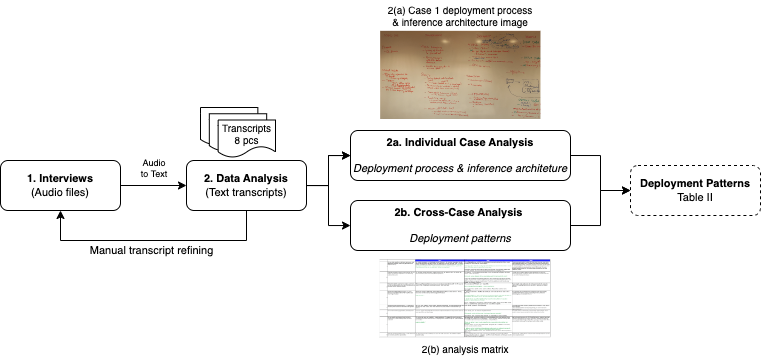
\includegraphics[width=0.9\textwidth]{images/data_analysis_process.png}
\caption{Data analysis process}
\label{fig: data analysis process}
\end{figure*}

%We further depicted each case's inference architecture with a diagram we later sent to the interviewees for validation.

% A straightforward research question concerned with how or why certain phenomena occur
% Case study research uses purposive sampling rather than random sampling
